\chapter{O organismo: um sistema em interação com o ambiente}\label{ch:b1:organism-environment}

Um coelho está parado na borda de um prado numa manhã de janeiro. Na
hora seguinte ele vai comer cem gramas de capim, respirar uns
\qty{400}{L} de ar, perder calor pela pelagem para um ar a
\qty{2}{\celsius}, beber de uma poça e disparar quando a sombra de um
gavião cruzar o campo. Nada do que ele faz é possível sem que algo
atravesse a fronteira dele: matéria que entra e sai, energia que entra e
sai, informação que entra. Duzentos metros adiante, um carvalho faz as
mesmas coisas sem se mover --- toma dióxido de carbono e luz, puxa água
por um sistema radicular maior que a copa e perde essa água para o mesmo
ar frio. Este capítulo enuncia o que é um \omterm{def:b1:organism-environment:organism}{organismo} enquanto sistema,
por que o tamanho dele dita como ele é construído, como ele mantém o
interior estável enquanto tudo lá fora muda, e como as necessidades
energéticas dele escalam com a massa. Os dois \omterm{def:b1:organism-environment:organism}{organismos} desta abertura,
um mamífero e uma planta com flores, são os modelos aos quais o ano
inteiro retorna.

\begin{omfigure}
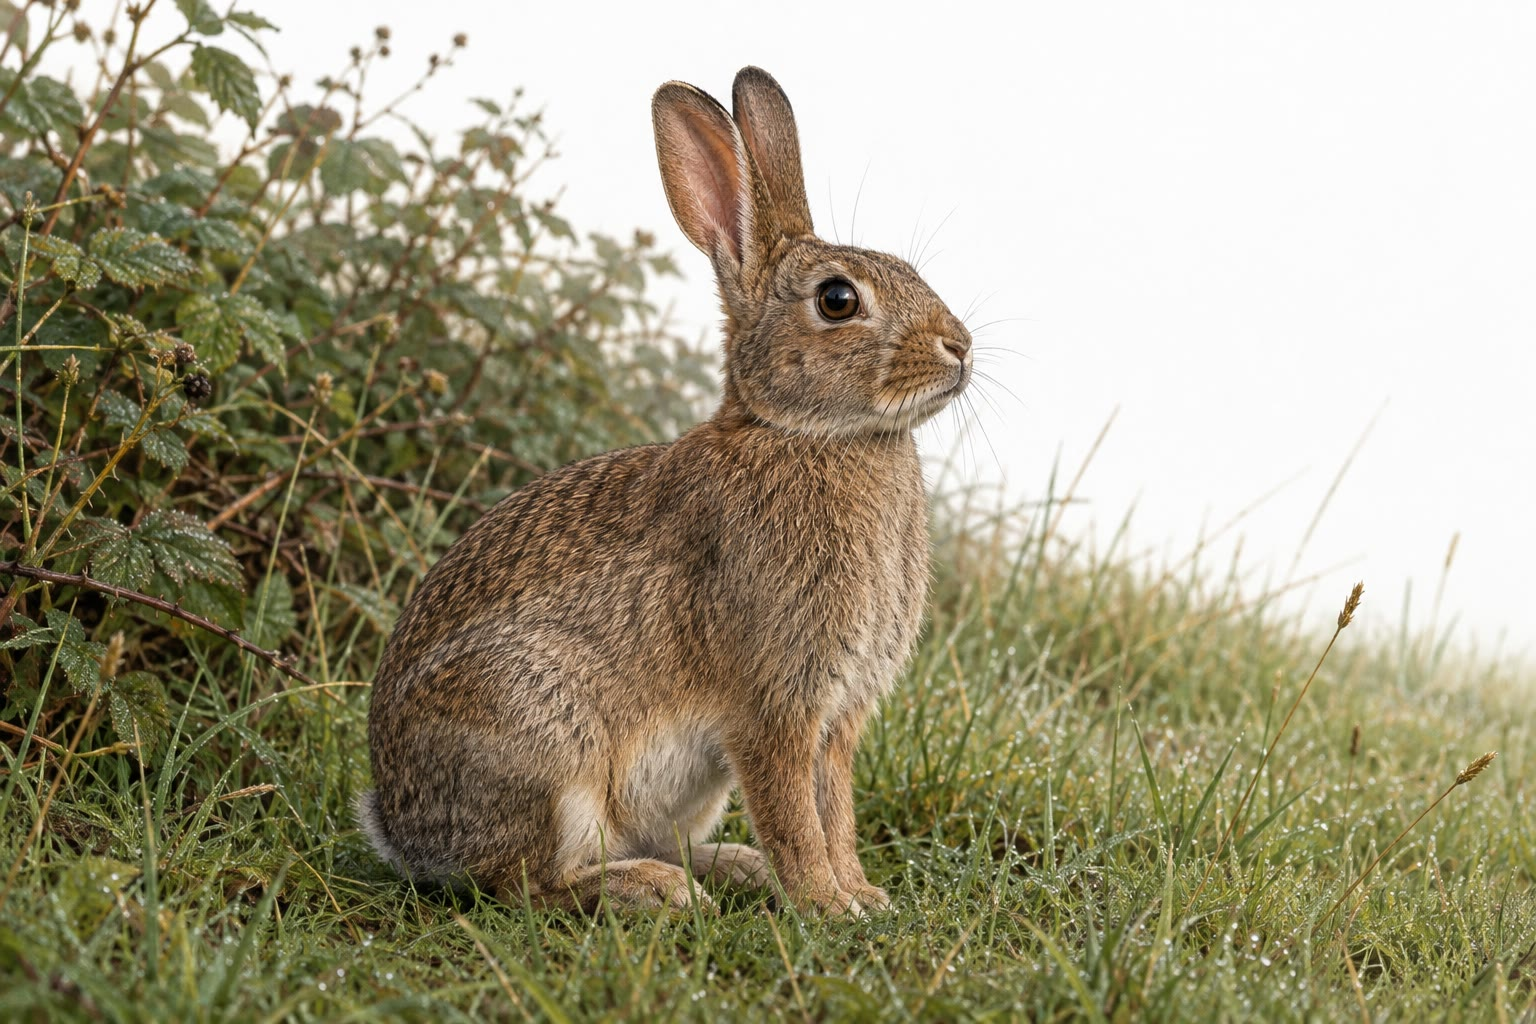
\includegraphics[width=0.62\linewidth]{images/book3/ai/b3-01-rabbit-field.jpg}

{\small Um coelho selvagem na borda de um prado: em uma hora ele vai
comer, respirar, perder calor, beber e fugir --- cada uma dessas coisas
uma troca através da fronteira dele.}
\end{omfigure}

\section{Um sistema aberto}

\begin{definition}[Organismo, sistema aberto]\label{def:b1:organism-environment:organism}
Um \emph{organismo}\index{organismo} é um indivíduo vivo: um sistema
delimitado, que se mantém e se reproduz por conta própria, feito de uma
célula ou de muitas células que compartilham uma origem comum e um
funcionamento comum. Ele é um \emph{sistema aberto}\index{sistema aberto}:
matéria e energia atravessam continuamente a fronteira dele, e ele só
permanece vivo enquanto isso acontece. O \emph{ambiente}\index{ambiente}
de um organismo é tudo o que está fora dessa fronteira e troca com ele
--- o meio físico (ar, água, solo, luz, temperatura) e os outros
organismos.
\end{definition}

\begin{proposition}[As três trocas]\label{prop:b1:organism-environment:exchanges}
Todo \omterm{def:b1:organism-environment:organism}{organismo} troca três coisas com o ambiente:
\begin{itemize}
  \item \emph{matéria}\index{troca de matéria}: ele absorve nutrientes,
        água e gases e libera dejetos, gases e água;
  \item \emph{energia}\index{troca de energia}: ele capta energia na
        forma de luz (autótrofos) ou na forma da energia química dos
        alimentos (heterótrofos), e a devolve quase inteiramente como
        calor;
  \item \emph{informação}\index{troca de informação}: ele detecta sinais
        do ambiente (luz, substâncias químicas, temperatura, tato, som)
        e responde a eles.
\end{itemize}
Ao longo de um período em que o \omterm{def:b1:organism-environment:organism}{organismo} não cresce nem encolhe, o
balanço dele fecha: a matéria que entra é igual à que sai, e a energia
que entra é igual ao calor que sai mais o trabalho realizado sobre o
exterior.
\end{proposition}
\begin{proof}
As duas primeiras decorrem da conservação da massa e da energia aplicada
ao volume interno à fronteira: o que se acumula é a diferença entre o
que entra e o que sai, e um \omterm{def:b1:organism-environment:organism}{organismo} em regime estacionário não acumula
nada. A energia química que não é armazenada como biomassa nova termina
como calor, porque toda reação do \omterm{def:b1:organism-environment:organism}{organismo} dissipa a energia livre dela
como calor, e o trabalho mecânico realizado sobre o exterior
(deslocar-se, levantar) é a única outra saída. A terceira é a
constatação de que nenhum \omterm{def:b1:organism-environment:organism}{organismo} é inerte diante do que o cerca.
\end{proof}

\begin{omfigure}
\begin{tikzpicture}[font=\footnotesize, >=Stealth, line cap=round]
  \draw[very thick, omDef, fill=omDef!6, rounded corners=12pt] (0,0) rectangle (4.4,3.4);
  \node[font=\small\bfseries, omDef] at (2.2,2.95) {organismo};
  \node[align=center] at (2.2,1.5) {meio interno\\ células, tecidos, órgãos\\ trabalho químico, crescimento,\\ movimento, reprodução};
  % matter in / out
  \draw[->, thick, omProp] (-1.3,2.6) -- (0,2.6) node[pos=0, left, align=right] {nutrientes, água,\\ $\mathrm{O_2}$ ou $\mathrm{CO_2}$};
  \draw[->, thick, omProp] (4.4,2.6) -- (5.7,2.6) node[right, align=left] {dejetos, água,\\ $\mathrm{CO_2}$ ou $\mathrm{O_2}$};
  % energy
  \draw[->, thick, omThm] (-1.3,1.5) -- (0,1.5) node[pos=0, left, align=right] {energia: luz, ou\\ energia química do alimento};
  \draw[->, thick, omThm] (4.4,1.5) -- (5.7,1.5) node[right, align=left] {calor, e o trabalho\\ realizado sobre o exterior};
  % information
  \draw[->, thick, omExo] (-1.3,0.5) -- (0,0.5) node[pos=0, left, align=right] {informação: luz,\\ substâncias, temperatura};
  \draw[->, thick, omExo] (4.4,0.5) -- (5.7,0.5) node[right, align=left] {respostas: movimento,\\ secreção, crescimento};
\end{tikzpicture}

{\small O \omterm{def:b1:organism-environment:organism}{organismo} como \omterm{def:b1:organism-environment:organism}{sistema aberto}: matéria (laranja), energia
(vermelho) e informação (verde) atravessam a fronteira dele. Um
\omterm{def:b1:organism-environment:organism}{organismo} em regime estacionário libera tanta matéria quanto absorve e
converte quase toda a energia que capta em calor.}
\end{omfigure}

\begin{definition}[Autótrofo, heterótrofo]\label{def:b1:organism-environment:trophy}
Um \omterm{def:b1:organism-environment:organism}{organismo} é \emph{autotrófico}\index{autotrofia} quando constrói a
própria matéria orgânica a partir de carbono mineral (dióxido de
carbono) usando uma fonte externa de energia --- a luz, no caso dos
\emph{fotoautótrofos}\index{fotoautótrofo} (plantas, algas,
cianobactérias), e a oxidação de compostos minerais, no caso dos
\emph{quimioautótrofos}\index{quimioautótrofo}. Ele é
\emph{heterotrófico}\index{heterotrofia} quando precisa absorver matéria
orgânica produzida por outros \omterm{def:b1:organism-environment:organism}{organismos}, que lhe fornece ao mesmo tempo
o carbono e a energia (animais, fungos, a maior parte das bactérias).
\end{definition}

\begin{example}[O coelho e o carvalho]\label{ex:b1:organism-environment:rabbitoak}
Os cem gramas de capim do coelho fornecem, uma vez digeridos, cerca de
\qty{500}{kJ} de energia química e o carbono de cada molécula que ele
vai construir; o oxigênio que ele respira lhe permite oxidar esse
alimento, e o dióxido de carbono que ele expira é esse mesmo carbono
saindo. A entrada do carvalho é o inverso: dióxido de carbono para
dentro, oxigênio para fora, a energia chegando como luz --- uns
\qty{5}{kW} incidindo sobre a copa ao meio-dia, dos quais ele armazena
menos de um por cento como açúcar. Os dois liberam como calor quase toda
a energia que processam: a pelagem do coelho é quente, e as folhas do
carvalho são resfriadas pela evaporação que a própria absorção de luz
delas impulsiona.
\end{example}

\section{Escalas de organização e o problema do tamanho}

\begin{definition}[Níveis de organização]\label{def:b1:organism-environment:levels}
A matéria viva é organizada em \emph{níveis de organização}\index{níveis de organização}
encaixados, cada um construído a partir das unidades do nível abaixo e
cada um com propriedades que o nível inferior não tem: moléculas
($\qty{1}{nm}$), células ($\qtyrange{1}{100}{\micro m}$), tecidos,
órgãos ($\qtyrange{1}{100}{mm}$), sistemas de órgãos, o \omterm{def:b1:organism-environment:organism}{organismo}
($\qty{1}{\micro m}$ a $\qty{100}{m}$), e acima dele a população, a
comunidade, o ecossistema e a biosfera. Uma célula respira; uma molécula
não. Uma população evolui; um \omterm{def:b1:organism-environment:organism}{organismo} não.
\end{definition}

\begin{proposition}[Superfície e volume]\label{prop:b1:organism-environment:sv}
Para corpos de mesma forma e de tamanho característico $L$, a superfície
cresce como $L^2$ e o volume como $L^3$, de modo que a razão
superfície/volume cai como $1/L$:
\[
\frac{S}{V} \propto \frac{1}{L}, \qquad
\frac{S}{V}\Big|_{\text{esfera}} = \frac{4\pi r^2}{\tfrac{4}{3}\pi r^3} = \frac{3}{r}.
\]
Tudo o que um \omterm{def:b1:organism-environment:organism}{organismo} troca atravessa uma superfície, e tudo o que ele
consome é proporcional ao volume dele: um \omterm{def:b1:organism-environment:organism}{organismo} grande não consegue
alimentar o próprio volume através da superfície externa.
\end{proposition}
\begin{proof}
Ampliar uma forma por um fator $k$ multiplica cada área por $k^2$ e cada
volume por $k^3$; a razão fica multiplicada por $1/k$. Para uma esfera a
fórmula é exata.
\end{proof}

\begin{example}[Uma bactéria e um ser humano]\label{ex:b1:organism-environment:svnumbers}
Uma bactéria de raio $\qty{0.5}{\micro m}$ tem
$S/V = 3/r = \qty{6e6}{m^{-1}}$: cada micrômetro cúbico do citoplasma
dela está a menos de meio micrômetro do exterior, e a difusão através da
membrana a alimenta por inteiro. Um ser humano modelado como uma esfera
de \qty{70}{L} tem $r = \qty{0.26}{m}$ e $S/V = \qty{12}{m^{-1}}$, meio
milhão de vezes menos. A pele, cerca de \qty{2}{m^2}, não conseguiria
fornecer o oxigênio que \qty{70}{kg} de tecido consomem; o pulmão,
dobrado dentro do tórax, oferece \qty{100}{m^2}, e o intestino, dobrado
três vezes sobre si mesmo, \qty{30}{m^2}.
\end{example}

\begin{omfigure}
\begin{tikzpicture}
\begin{axis}[
  xbar, bar width=8pt,
  width=0.78\linewidth, height=6.2cm,
  axis x line=bottom, axis y line=left,
  xmode=log, log origin=infty, xmin=0.5, xmax=3000,
  xlabel={superfície de troca (\unit{m^2})},
  xlabel style={font=\small, at={(axis description cs:0.5,-0.13)}, anchor=north},
  symbolic y coords={pele humana, pulmão humano, intestino delgado humano, folhas de carvalho, sistema radicular do centeio, pelos radiculares do centeio},
  ytick=data, tick label style={font=\small},
  enlarge y limits=0.12,
  nodes near coords, nodes near coords style={font=\scriptsize, anchor=west},
  point meta=rawx,
]
\addplot[fill=omDef!45, draw=omDef] coordinates
  {(2,pele humana) (100,pulmão humano) (30,intestino delgado humano) (300,folhas de carvalho) (240,sistema radicular do centeio) (400,pelos radiculares do centeio)};
\end{axis}
\end{tikzpicture}

{\small \omterm{prop:b1:organism-environment:surfaces}{Superfícies de troca}, em escala logarítmica. A superfície
externa de um ser humano é de \qty{2}{m^2}; as superfícies dobradas
dentro dele, e as superfícies que uma planta espalha pelo ar e pelo
solo, são de dez a duzentas vezes maiores. (Um único pé de centeio
cultivado quatro meses num vaso: \qty{240}{m^2} de raízes e
\qty{400}{m^2} de pelos radiculares.)}
\end{omfigure}

\begin{proposition}[As superfícies de troca são dobradas, finas e ventiladas]\label{prop:b1:organism-environment:surfaces}
Acima de um tamanho da ordem do milímetro, um \omterm{def:b1:organism-environment:organism}{organismo} não pode ser
alimentado por difusão através da superfície externa. Os \omterm{def:b1:organism-environment:organism}{organismos}
pluricelulares de qualquer tamanho carregam por isso
\emph{superfícies de troca especializadas}\index{superfície de troca}, cujo desenho comum resolve o mesmo problema de quatro maneiras: uma
área grande (dobramento: vilosidades, alvéolos, lamelas branquiais,
pelos radiculares, lâminas foliares), uma espessura pequena (uma camada
de células ou menos entre os dois meios), um meio renovado do lado de
fora (ventilação, corrente de água, corrente de transpiração) e um
sistema de transporte do lado de dentro (sangue, seiva) que leva ao
resto do volume o que atravessa a superfície.
\end{proposition}
\begin{proof}
A lei de Fick (\cref{ch:b1:membranes-transport}) dá o fluxo através de
uma superfície como proporcional à área, à diferença de concentração e
ao inverso da espessura; renovar o meio externo mantém grande a
diferença de concentração; um sistema de transporte retira o que
atravessou e mantém baixa a concentração interna. Cada uma das quatro
características aumenta o fluxo; um \omterm{def:b1:organism-environment:organism}{organismo} grande precisa das quatro.
\end{proof}

\section{O meio interno e a homeostase}

\begin{definition}[Meio interno]\label{def:b1:organism-environment:milieu}
Num animal pluricelular a maior parte das células não está em contato
com o mundo exterior, e sim banhada em um \emph{meio interno}\index{meio interno}: o líquido extracelular (plasma sanguíneo, linfa, o líquido
intersticial entre as células) cuja composição, temperatura e volume o
\omterm{def:b1:organism-environment:organism}{organismo} regula. As células trocam com esse líquido; o líquido troca
com o exterior através das superfícies especializadas. A ideia é de
Claude Bernard (1865): a constância do meio interno é a condição de uma
vida livre e independente.
\end{definition}

\begin{definition}[Homeostase]\label{def:b1:organism-environment:homeostasis}
\emph{Homeostase}\index{homeostase} é a manutenção de uma variável
regulada do \omterm{def:b1:organism-environment:milieu}{meio interno} (temperatura, concentração de glicose, pH,
osmolaridade, pressão arterial) próxima de um
\emph{valor de referência}\index{valor de referência} apesar das
mudanças externas. Ela é obtida por
\emph{retroalimentação negativa}\index{retroalimentação negativa}: um
\emph{sensor} mede a variável, um centro integrador a compara com o
valor de referência, e um \emph{efetor} age no sentido que anula o
desvio. A variável não fica fixa: ela oscila numa faixa estreita em
torno do valor de referência.
\end{definition}

\begin{omfigure}
\begin{tikzpicture}[font=\small, >=Stealth, line cap=round,
  box/.style={draw, thick, rounded corners=4pt, minimum height=9mm, minimum width=26mm, align=center, fill=white}]
  \node[box, fill=omDef!10] (var) at (0,0) {variável regulada\\ (por exemplo, a temperatura corporal)};
  \node[box, fill=omProp!10] (sens) at (4.6,1.5) {sensor\\ (termorreceptores)};
  \node[box, fill=omThm!10] (int) at (4.6,-1.5) {centro integrador\\ (hipotálamo)};
  \node[box, fill=omExo!10] (eff) at (0,-3.0) {efetores\\ (tremor, vasos, suor)};
  \node[font=\footnotesize, align=center] (set) at (8.4,-1.5) {valor de referência\\ $\qty{37}{\celsius}$};
  \draw[->, thick] (var.east) -- ++(1.0,0) |- (sens.west);
  \draw[->, thick] (sens.south) -- (int.north) node[midway, right, font=\footnotesize] {valor medido};
  \draw[->, thick] (set.west) -- (int.east);
  \draw[->, thick] (int.south) -- ++(0,-0.6) -| (eff.east) ;
  \draw[->, thick] (eff.north) -- (var.south) node[midway, left, font=\footnotesize, align=right] {correção,\\ oposta ao desvio};
  \draw[->, thick, gray] (-3.6,0.9) -- (var.north west) node[pos=0, above, font=\footnotesize, gray, align=center] {perturbação\\ (ar frio)};
\end{tikzpicture}

{\small Uma alça de \omterm{def:b1:organism-environment:homeostasis}{retroalimentação negativa}. O sensor informa a
variável, o centro a compara com o \omterm{def:b1:organism-environment:homeostasis}{valor de referência} e os efetores
empurram a variável de volta. O sinal da correção é sempre oposto ao do
desvio --- daí \emph{negativa}.}
\end{omfigure}

\begin{proposition}[Endotermos e ectotermos]\label{prop:b1:organism-environment:thermo}
Um \emph{ectotermo}\index{ectotermo} (a maioria dos invertebrados, os
peixes, os anfíbios, os répteis) tem uma temperatura corporal que
acompanha a do ambiente; a \omterm{def:b1:organism-environment:allometry}{taxa metabólica} dele sobe com a temperatura,
dobrando aproximadamente a cada \qty{10}{\celsius}. Um
\emph{endotermo}\index{endotermo} (mamíferos, aves) mantém a
temperatura corporal em um \omterm{def:b1:organism-environment:homeostasis}{valor de referência} produzindo calor
metabolicamente. Dentro de uma
\emph{zona de termoneutralidade}\index{zona de termoneutralidade} de
temperaturas ambientes ele o faz com a taxa basal, ajustando apenas o
isolamento e o fluxo de sangue para a pele; abaixo dessa zona a \omterm{def:b1:organism-environment:allometry}{taxa
metabólica} dele sobe linearmente à medida que o ar esfria, porque a
perda de calor é proporcional à diferença de temperatura e precisa ser
compensada pela produção de calor; acima dela, resfriar-se por
evaporação custa água e energia.
\end{proposition}
\begin{proof}[Demonstração parcial]
Para um corpo a $T_b$ em ar a $T_a$, o calor perdido por unidade de
tempo através da superfície dele é $P = hS\,(T_b - T_a)$ (lei do
resfriamento de Newton), com $h$ um coeficiente reduzido por pelo, penas
ou gordura. Uma temperatura estacionária exige uma produção de calor
igual a $P$, portanto linear em $T_a$ abaixo da \omterm{prop:b1:organism-environment:thermo}{zona de
termoneutralidade}, com inclinação $-hS$. A existência e a largura da
zona, em que o próprio $h$ é ajustado (eriçar o pelo, contrair os vasos
da pele), são fatos fisiológicos, e não consequências da equação.
\end{proof}

\begin{omfigure}
\begin{tikzpicture}
\begin{axis}[
  width=0.9\linewidth, height=6.4cm,
  axis x line=bottom, axis y line=left,
  xmin=-10, xmax=45, ymin=0, ymax=5.2,
  xlabel={temperatura ambiente (\unit{\celsius})}, ylabel={taxa metabólica (múltiplos da basal)},
  xlabel style={font=\small, at={(axis description cs:0.5,-0.12)}, anchor=north},
  ylabel style={font=\small},
  tick label style={font=\small}, xtick={-10,0,10,20,30,40}, ytick={1,2,3,4,5},
  clip=false, legend style={font=\small, at={(0.97,0.97)}, anchor=north east, draw=none},
]
\addplot[very thick, omThm] coordinates {(-10,4.6) (0,3.4) (10,2.2) (20,1.0) (30,1.0) (33,1.05) (38,1.5) (42,2.2)};
\addlegendentry{endotermo (um camundongo)}
\addplot[very thick, omDef] coordinates {(-10,0.05) (0,0.12) (10,0.25) (20,0.5) (30,1.0) (40,2.0)};
\addlegendentry{ectotermo (um lagarto)}
\draw[dashed, gray] (axis cs:20,0) -- (axis cs:20,1.0);
\draw[dashed, gray] (axis cs:30,0) -- (axis cs:30,1.0);
\node[font=\scriptsize, anchor=south, align=center] at (axis cs:25,1.15) {zona de\\ termoneutralidade};
\node[font=\scriptsize, anchor=west, align=left] at (axis cs:11,3.5) {inclinação $= -hS$: a produção de calor\\ compensa a perda};
\end{axis}
\end{tikzpicture}

{\small \omterm{def:b1:organism-environment:allometry}{Taxa metabólica} em função da temperatura ambiente. A taxa do
\omterm{prop:b1:organism-environment:thermo}{endotermo} é mínima na \omterm{prop:b1:organism-environment:thermo}{zona de termoneutralidade} dele e sobe linearmente
à medida que o ar esfria; a taxa do \omterm{prop:b1:organism-environment:thermo}{ectotermo} simplesmente acompanha a
temperatura, dobrando a cada dez graus.}
\end{omfigure}

\begin{example}[Uma noite a dois graus]\label{ex:b1:organism-environment:night}
O coelho da abertura, em repouso na toca, produz cerca de \qty{6}{W} de
calor dentro da \omterm{prop:b1:organism-environment:thermo}{zona de termoneutralidade} dele. Lá fora, a
\qty{2}{\celsius}, vinte graus abaixo da borda inferior dessa zona, a
produção dele precisa subir para cerca de \qty{12}{W}: o tremor e a
oxidação das reservas de gordura fornecem a diferença, e o tempo que ele
passa se alimentando aumenta. O lagarto na mesma margem não luta contra
o frio: o corpo dele cai a \qty{3}{\celsius}, o metabolismo cai a um
vigésimo do valor de verão, e ele não se move até o sol voltar.
\end{example}

\section{Taxa metabólica e massa corporal}

\begin{definition}[Taxa metabólica, alometria]\label{def:b1:organism-environment:allometry}
A \emph{taxa metabólica}\index{taxa metabólica} $B$ de um \omterm{def:b1:organism-environment:organism}{organismo} é a
taxa com que ele converte energia química, medida em watts como produção
de calor ou como consumo de oxigênio ($\qty{1}{L}$ de $\mathrm{O_2}$
consumido $\approx \qty{20}{kJ}$). A
\emph{taxa metabólica basal}\index{taxa metabólica basal} é a de um
\omterm{prop:b1:organism-environment:thermo}{endotermo} em repouso e em jejum, dentro da \omterm{prop:b1:organism-environment:thermo}{zona de termoneutralidade}
dele. Diz-se que uma grandeza $Y$ escala
\emph{alometricamente}\index{alometria} com a massa corporal $M$ quando
$Y = a\,M^{b}$ com um expoente $b \neq 1$; num gráfico log--log a
relação é uma reta de inclinação $b$.
\end{definition}

\begin{theorem}[Lei de Kleiber]\label{thm:b1:organism-environment:kleiber}
\index{lei de Kleiber}
Entre os mamíferos e as aves, de um musaranho a uma baleia, a \omterm{def:b1:organism-environment:allometry}{taxa
metabólica basal} escala com a potência três quartos da massa corporal:
\[
B \approx \qty{3.4}{W}\times\left(\frac{M}{\qty{1}{kg}}\right)^{3/4}.
\]
A taxa \emph{específica por massa} $B/M$ cai, portanto, como $M^{-1/4}$:
cada grama de um camundongo queima energia cerca de vinte vezes mais
rápido que cada grama de um elefante.
\end{theorem}
\begin{proof}[Evidências]
Kleiber (1932) representou a produção de calor medida em animais de
\qty{20}{g} a \qty{600}{kg} contra a massa deles em eixos logarítmicos e
encontrou uma reta de inclinação $0.74$, e não o $0.67$ que uma perda de
calor proporcional à superfície preveria. A reta foi desde então
estendida por oito ordens de grandeza em massa, com a mesma inclinação a
menos de alguns centésimos. Por que o expoente é $3/4$ e não $2/3$ segue
em debate: a explicação dominante o liga à geometria das redes
ramificadas (vasos, vias aéreas) que entregam oxigênio a cada célula.
\end{proof}

\begin{omfigure}
\begin{tikzpicture}
\begin{loglogaxis}[
  width=0.9\linewidth, height=6.6cm,
  axis x line=bottom, axis y line=left,
  xmin=0.005, xmax=20000, ymin=0.05, ymax=6000,
  xlabel={massa corporal (\unit{kg})}, ylabel={taxa metabólica basal (\unit{W})},
  xlabel style={font=\small, at={(axis description cs:0.5,-0.12)}, anchor=north},
  ylabel style={font=\small},
  tick label style={font=\small},
  xtick={0.01,0.1,1,10,100,1000,10000}, ytick={0.1,1,10,100,1000},
  log ticks with fixed point,
  clip=false,
]
\addplot[thick, omThm, domain=0.005:20000, samples=40] {3.4*x^0.75};
\addplot[only marks, mark=*, mark size=2pt, omDef] coordinates
  {(0.02,0.19) (0.3,1.3) (3,7.5) (70,80) (500,360) (4000,1700)};
\node[font=\scriptsize, anchor=west] at (axis cs:0.02,0.19) {\ camundongo};
\node[font=\scriptsize, anchor=west] at (axis cs:0.3,1.3) {\ rato};
\node[font=\scriptsize, anchor=west] at (axis cs:3,7.5) {\ gato};
\node[font=\scriptsize, anchor=west] at (axis cs:70,80) {\ ser humano};
\node[font=\scriptsize, anchor=west] at (axis cs:500,360) {\ cavalo};
\node[font=\scriptsize, anchor=north] at (axis cs:4000,1300) {elefante};
\node[font=\scriptsize, anchor=south east, omThm] at (axis cs:8000,4000) {inclinação $3/4$};
\end{loglogaxis}
\end{tikzpicture}

{\small A \omterm{thm:b1:organism-environment:kleiber}{lei de Kleiber}. \omterm{def:b1:organism-environment:allometry}{Taxa metabólica basal} em função da massa
corporal para seis mamíferos em eixos logarítmicos: os pontos caem sobre
uma reta de inclinação $3/4$ ao longo de cinco ordens de grandeza de
massa.}
\end{omfigure}

\begin{method}[Como ler um gráfico alométrico]\label{met:b1:organism-environment:loglog}
\begin{enumerate}
  \item Represente $\log Y$ contra $\log M$ (ou use eixos logarítmicos).
        Uma lei de potência $Y = aM^b$ vira a reta
        $\log Y = \log a + b\log M$.
  \item O expoente $b$ é a inclinação: tome dois pontos separados por
        uma década em $M$; $b$ é o número de décadas que $Y$ subiu. Um
        expoente igual a $1$ significa proporcionalidade (isometria);
        $b < 1$, a grandeza cresce mais devagar que a massa; $b > 1$,
        mais rápido.
  \item O prefator $a$ é o valor de $Y$ em $M = 1$ (onde $\log M = 0$).
  \item Para comparar dois \omterm{def:b1:organism-environment:organism}{organismos}, use a razão: $Y_2/Y_1 =
        (M_2/M_1)^b$. Por unidade de massa, o expoente vira $b-1$.
\end{enumerate}
\end{method}

\begin{example}[Camundongo e elefante]\label{ex:b1:organism-environment:mouseelephant}
Um camundongo de \qty{20}{g}: $B = 3.4\times 0.02^{0.75} = \qty{0.18}{W}$,
ou \qty{9}{W/kg}. Um elefante de \qty{4}{t}: $B = 3.4\times 4000^{0.75} =
\qty{1700}{W}$, ou \qty{0.43}{W/kg}. O elefante queima dez mil vezes
mais que o camundongo, mas cada grama dele queima vinte e uma vezes
menos: $(4000/0.02)^{-1/4} = 1/21$. O camundongo precisa comer um
décimo da própria massa por dia; o elefante, um quinquagésimo. O
coração do camundongo bate \qty{600}{} vezes por minuto, o do elefante
\qty{30}{}: a frequência cardíaca, como $B/M$, escala como $M^{-1/4}$,
e os corações dos dois animais batem cerca de um bilhão de vezes ao
longo da vida.
\end{example}

\begin{remark}[Dois expoentes de escala, e o que decorre deles]\label{rem:b1:organism-environment:consequences}
Muitas taxas de um \omterm{def:b1:organism-environment:organism}{organismo} escalam como $M^{-1/4}$ (frequência
cardíaca, frequência respiratória, metabolismo específico por massa) e
muitos tempos como $M^{+1/4}$ (longevidade, gestação, tempo até a
maturidade); os produtos deles, como o número de batimentos por vida,
são então independentes da massa. Os tamanhos dos órgãos escalam perto
de $M^{1}$ (coração, pulmão e volume de sangue são uma fração fixa do
corpo), enquanto as superfícies através das quais eles trocam escalam
como $M^{3/4}$ --- e é por isso que o pulmão de um animal grande é mais
finamente dobrado que o de um pequeno, e não apenas maior.
\end{remark}

\section{Dois organismos-modelo}

\begin{proposition}[Um mamífero e uma planta com flores]\label{prop:b1:organism-environment:models}
Os dois \omterm{def:b1:organism-environment:organism}{organismos} pluricelulares que este ano usa como modelos resolvem
os problemas acima de maneiras opostas. Um mamífero é um heterótrofo
móvel com um \omterm{def:b1:organism-environment:milieu}{meio interno} regulado: ele obtém matéria e energia
procurando e comendo alimento, troca através de superfícies internas
(intestino, pulmão, rim) irrigadas por uma circulação, mantém
constantes a temperatura e a composição do sangue, e chega a uma forma
adulta fixa. Uma planta com flores é um \omterm{def:b1:organism-environment:trophy}{fotoautótrofo} fixo com um corpo
aberto e modular: ela obtém energia e carbono da luz e do ar nas folhas,
e água e minerais do solo nas raízes, troca através de superfícies
externas que vai ampliando por crescimento ao longo da vida inteira, não
regula a própria temperatura e ajusta a forma ao local. Os dois
capítulos seguintes descrevem cada um deles.
\end{proposition}

\begin{example}[A mesma hora, dois balanços]\label{ex:b1:organism-environment:budgets}
Na hora da abertura, o coelho transformou \qty{500}{kJ} de capim em
calor, movimento e um pouco de crescimento, mantendo o sangue a
\qty{39}{\celsius} e a glicose perto de \qty{6}{mmol/L}; ele o fez indo
até o alimento. O carvalho transformou algumas centenas de quilojoules
da luz solar sobre a copa em açúcar, perdeu \qty{5}{L} de água pelas
folhas para fazê-lo, e produziu alguns micrômetros de madeira nova; ele
o fez estando onde estavam a luz e a água. Os dois são \omterm{def:b1:organism-environment:organism}{sistemas abertos};
os dois se mantêm trocando; as formas das trocas deles são as formas das
vidas deles.
\end{example}

\section{Exercícios}

\begin{exercise}[$\star$]\label{exo:b1:organism-environment:1}
Cite os três tipos de troca entre um \omterm{def:b1:organism-environment:organism}{organismo} e o ambiente dele, com um
exemplo de cada um para um mamífero e um para uma planta.
\end{exercise}

\begin{exercise}[$\star$]\label{exo:b1:organism-environment:2}
Diga o que acontece com a razão superfície/volume quando uma célula
esférica dobra o raio, e por que isso limita o tamanho celular.
\end{exercise}

\begin{exercise}[$\star$]\label{exo:b1:organism-environment:3}
Defina \omterm{def:b1:organism-environment:homeostasis}{homeostase} e cite os três componentes de uma alça de
\omterm{def:b1:organism-environment:homeostasis}{retroalimentação negativa}, com a identidade de cada um na regulação da
temperatura corporal.
\end{exercise}

\begin{exercise}[$\star$]\label{exo:b1:organism-environment:4}
A partir da figura das \omterm{def:b1:organism-environment:allometry}{taxas metabólicas}, por qual fator a \omterm{def:b1:organism-environment:allometry}{taxa
metabólica} do lagarto cai entre \qty{30}{\celsius} e
\qty{10}{\celsius}, e por qual fator a do camundongo sobe entre
\qty{20}{\celsius} e \qty{0}{\celsius}?
\end{exercise}

\begin{exercise}[$\star\star$]\label{exo:b1:organism-environment:5}
Um \omterm{def:b1:organism-environment:organism}{organismo} em forma de cubo com aresta de \qty{1}{mm} precisa de
\qty{1}{nmol} de oxigênio por segundo e por milímetro cúbico, e a
superfície dele consegue captar no máximo \qty{2}{nmol/s} por milímetro
quadrado. Ele pode viver por difusão através da superfície? Repita para
uma aresta de \qty{10}{mm}. Encontre a maior aresta que consegue.
\end{exercise}

\begin{exercise}[$\star\star$]\label{exo:b1:organism-environment:6}
Usando a \omterm{thm:b1:organism-environment:kleiber}{lei de Kleiber}, calcule a \omterm{def:b1:organism-environment:allometry}{taxa metabólica basal} de um cavalo de
\qty{500}{kg} e de um musaranho de \qty{5}{g}, e a taxa específica por
massa de cada um. Quantas vezes a própria massa em alimento, a
\qty{5}{kJ/g}, o musaranho precisa comer por dia se o gasto diário dele
é três vezes a taxa basal?
\end{exercise}

\begin{exercise}[$\star\star$]\label{exo:b1:organism-environment:7}
Um ser humano em repouso produz \qty{80}{W}. Converta isso em litros de
oxigênio consumidos por minuto e em quilojoules por dia. Uma dieta de
\qty{2000}{kcal} corresponde a quantos watts? (\qty{1}{kcal} =
\qty{4.18}{kJ}.)
\end{exercise}

\begin{exercise}[$\star\star$]\label{exo:b1:organism-environment:8}
O pulmão de um ser humano de \qty{70}{kg} tem uma \omterm{prop:b1:organism-environment:surfaces}{superfície de troca}
de cerca de \qty{100}{m^2}. Se a superfície pulmonar escalasse com a
massa corporal elevada a $3/4$, que superfície teria o pulmão de um
camundongo de \qty{20}{g}, e o de um elefante de \qty{4000}{kg}?
Compare com a superfície de uma esfera do volume do animal (densidade
\qty{1000}{kg/m^3}).
\end{exercise}

\begin{exercise}[$\star\star$]\label{exo:b1:organism-environment:9}
Uma alça de \omterm{def:b1:organism-environment:homeostasis}{retroalimentação negativa} não consegue manter uma variável
exatamente no \omterm{def:b1:organism-environment:homeostasis}{valor de referência} dela. Explique por quê, usando a alça
da temperatura, e diga o que determina a largura da faixa dentro da qual
a variável oscila.
\end{exercise}

\begin{exercise}[$\star\star\star$]\label{exo:b1:organism-environment:10}
Um corpo perde calor à taxa $P = hS(T_b - T_a)$ com
$h = \qty{5}{W.m^{-2}.K^{-1}}$ para um mamífero com pelo. Para um
camundongo de \qty{20}{g} modelado como uma esfera de densidade
\qty{1000}{kg/m^3}, calcule a superfície, a perda de calor a
$T_a = \qty{0}{\celsius}$ com $T_b =
\qty{37}{\celsius}$, e compare com a taxa basal dele dada pela \omterm{thm:b1:organism-environment:kleiber}{lei de
Kleiber}. O que o camundongo precisa fazer?
\end{exercise}

\begin{exercise}[$\star\star\star$]\label{exo:b1:organism-environment:11}
Se a perda de calor escalasse com a superfície ($M^{2/3}$) e a produção
de calor com a \omterm{thm:b1:organism-environment:kleiber}{lei de Kleiber} ($M^{3/4}$), mostre que os menores
\omterm{prop:b1:organism-environment:thermo}{endotermos} são os que mais sofrem no frio, e que acima de certa massa um
animal teria dificuldade para perder calor. Estime, com
$h = \qty{5}{W.m^{-2}.K^{-1}}$ e $T_b - T_a = \qty{20}{K}$, a massa em
que a produção basal iguala a perda para um corpo esférico.
\end{exercise}

\begin{exercise}[$\star\star\star$]\label{exo:b1:organism-environment:12}
``Como uma planta não regula a temperatura nem os fluidos internos dela,
ela é um sistema mais simples que um animal.'' Discuta em um parágrafo,
usando as duas estratégias de troca deste capítulo, as superfícies que
cada uma usa, e o significado de \omterm{def:b1:organism-environment:homeostasis}{homeostase}.
\end{exercise}

\section{Problema: O camundongo e o elefante}

\begin{problem}[{Problema de fim de semana --- dois mamíferos separados
por cinco ordens de grandeza: as superfícies, o calor, o alimento, os
corações e os anos deles, terminando na razão que a lei de Kleiber prevê}]
\label{pb:b1:organism-environment:1}
Um camundongo doméstico tem massa de \qty{20}{g}; um elefante africano,
\qty{4000}{kg}. Os dois mantêm uma temperatura corporal perto de
\qty{37}{\celsius}, e os dois são modelados, quando é preciso uma forma,
como esferas de densidade \qty{1000}{kg/m^3}. A \omterm{thm:b1:organism-environment:kleiber}{lei de Kleiber} é
$B = \qty{3.4}{W}\,(M/\qty{1}{kg})^{3/4}$.

\medskip
\noindent\textbf{Parte I --- Geometria.}
\begin{enumerate}
  \item Calcule o volume de cada animal.
  \item Calcule o raio da esfera equivalente de cada um.
  \item Calcule a superfície de cada esfera.
  \item Calcule a razão superfície/volume de cada um, e a razão entre
        elas.
  \item Mostre que essa razão é igual à raiz cúbica da razão entre as
        massas, e verifique numericamente.
  \item Camundongos e elefantes reais não são esferas. Diga, com uma
        justificativa, se a razão superfície/volume real de cada um é
        maior ou menor que a da esfera, e qual animal se afasta mais.
\end{enumerate}

\medskip
\noindent\textbf{Parte II --- Calor.}
O calor é perdido pela superfície à taxa $P = hS\,(T_b - T_a)$. Tome
$h = \qty{10}{W.m^{-2}.K^{-1}}$ para pele nua e $T_a =
\qty{17}{\celsius}$.
\begin{enumerate}[resume]
  \item Calcule a perda de calor de cada esfera nua.
  \item Calcule a \omterm{def:b1:organism-environment:allometry}{taxa metabólica basal} de cada um pela \omterm{thm:b1:organism-environment:kleiber}{lei de Kleiber}.
  \item Compare perda e produção para o elefante. A pele nua é um
        problema para ele?
  \item Compare perda e produção para o camundongo. Que valor de $h$ a
        pelagem dele teria de fornecer para que a produção basal
        cobrisse a perda?
  \item As orelhas de um elefante acrescentam \qty{4}{m^2} de
        superfície fina e ricamente irrigada, e ele as abana no calor.
        Explique para que elas servem, usando a Parte I.
  \item Explique por que não existe \omterm{prop:b1:organism-environment:thermo}{endotermo} menor que alguns gramas, e
        por que os menores (musaranhos, beija-flores) deixam a
        temperatura cair à noite.
\end{enumerate}

\medskip
\noindent\textbf{Parte III --- Alimento.}
Um animal em vida livre gasta cerca do dobro da taxa basal ao longo de
um dia. As sementes do camundongo fornecem \qty{18}{kJ} por grama; o
capim fresco do elefante, \qty{5}{kJ} de energia digestível por grama.
\begin{enumerate}[resume]
  \item Calcule o gasto energético diário de cada um em quilojoules.
  \item Calcule a ingestão diária de alimento de cada um em gramas.
  \item Expresse cada ingestão como fração da massa corporal, e compare.
  \item O intestino do elefante tem cerca de \qty{35}{m} de comprimento
        e o do camundongo \qty{40}{cm}. Calcule a razão entre os
        comprimentos do intestino e compare-a com a razão entre os
        comprimentos corporais (os raios da Parte I). O que a comparação
        sugere sobre a escala do intestino?
\end{enumerate}

\medskip
\noindent\textbf{Parte IV --- Corações e anos.}
A frequência cardíaca escala como $f = f_0\,(M/\qty{1}{kg})^{-1/4}$, e a
longevidade como $\tau = \tau_0\,(M/\qty{1}{kg})^{1/4}$. O coração do
camundongo bate \qty{600}{} vezes por minuto e ele vive dois anos.
\begin{enumerate}[resume]
  \item Calcule $f_0$ e $\tau_0$ a partir do camundongo.
  \item Preveja a frequência cardíaca e a longevidade do elefante.
  \item Calcule o número de batimentos cardíacos na vida de cada animal.
  \item Explique, a partir dos dois expoentes, por que esse número é o
        mesmo.
  \item Preveja a frequência cardíaca e a longevidade de um ser humano
        de \qty{70}{kg} com as mesmas fórmulas, e compare com os valores
        reais (\qty{70}{} batimentos por minuto, uns \qty{80}{} anos).
        Qual previsão falha, e qual pode ser a razão?
  \item A frequência respiratória escala como a cardíaca. O camundongo
        respira \qty{160}{} vezes por minuto; preveja a frequência
        respiratória do elefante e calcule o número de batimentos
        cardíacos por respiração de cada um.
  \item Escreva a \omterm{def:b1:organism-environment:allometry}{taxa metabólica} específica por massa $B/M$ como uma
        potência de $M$ e dê o expoente dela.
  \item Calcule $B/M$ para o camundongo e para o elefante.
  \item Enuncie o resultado: a razão entre a \omterm{def:b1:organism-environment:allometry}{taxa metabólica} específica
        por massa do camundongo e a do elefante, e a potência da razão
        entre as massas a que ela é igual.
\end{enumerate}
\end{problem}
